\documentclass[twoside]{book}

% Packages required by doxygen
\usepackage{fixltx2e}
\usepackage{calc}
\usepackage{doxygen}
\usepackage{graphicx}
\usepackage[utf8]{inputenc}
\usepackage{makeidx}
\usepackage{multicol}
\usepackage{multirow}
\PassOptionsToPackage{warn}{textcomp}
\usepackage{textcomp}
\usepackage[nointegrals]{wasysym}
\usepackage[table]{xcolor}

% Font selection
\usepackage[T1]{fontenc}
\usepackage{mathptmx}
\usepackage[scaled=.90]{helvet}
\usepackage{courier}
\usepackage{amssymb}
\usepackage{sectsty}
\renewcommand{\familydefault}{\sfdefault}
\allsectionsfont{%
  \fontseries{bc}\selectfont%
  \color{darkgray}%
}
\renewcommand{\DoxyLabelFont}{%
  \fontseries{bc}\selectfont%
  \color{darkgray}%
}
\newcommand{\+}{\discretionary{\mbox{\scriptsize$\hookleftarrow$}}{}{}}

% Page & text layout
\usepackage{geometry}
\geometry{%
  a4paper,%
  top=2.5cm,%
  bottom=2.5cm,%
  left=2.5cm,%
  right=2.5cm%
}
\tolerance=750
\hfuzz=15pt
\hbadness=750
\setlength{\emergencystretch}{15pt}
\setlength{\parindent}{0cm}
\setlength{\parskip}{0.2cm}
\makeatletter
\renewcommand{\paragraph}{%
  \@startsection{paragraph}{4}{0ex}{-1.0ex}{1.0ex}{%
    \normalfont\normalsize\bfseries\SS@parafont%
  }%
}
\renewcommand{\subparagraph}{%
  \@startsection{subparagraph}{5}{0ex}{-1.0ex}{1.0ex}{%
    \normalfont\normalsize\bfseries\SS@subparafont%
  }%
}
\makeatother

% Headers & footers
\usepackage{fancyhdr}
\pagestyle{fancyplain}
\fancyhead[LE]{\fancyplain{}{\bfseries\thepage}}
\fancyhead[CE]{\fancyplain{}{}}
\fancyhead[RE]{\fancyplain{}{\bfseries\leftmark}}
\fancyhead[LO]{\fancyplain{}{\bfseries\rightmark}}
\fancyhead[CO]{\fancyplain{}{}}
\fancyhead[RO]{\fancyplain{}{\bfseries\thepage}}
\fancyfoot[LE]{\fancyplain{}{}}
\fancyfoot[CE]{\fancyplain{}{}}
\fancyfoot[RE]{\fancyplain{}{\bfseries\scriptsize Generated on Fri Mar 22 2019 13\+:17\+:57 for My Project by Doxygen }}
\fancyfoot[LO]{\fancyplain{}{\bfseries\scriptsize Generated on Fri Mar 22 2019 13\+:17\+:57 for My Project by Doxygen }}
\fancyfoot[CO]{\fancyplain{}{}}
\fancyfoot[RO]{\fancyplain{}{}}
\renewcommand{\footrulewidth}{0.4pt}
\renewcommand{\chaptermark}[1]{%
  \markboth{#1}{}%
}
\renewcommand{\sectionmark}[1]{%
  \markright{\thesection\ #1}%
}

% Indices & bibliography
\usepackage{natbib}
\usepackage[titles]{tocloft}
\setcounter{tocdepth}{3}
\setcounter{secnumdepth}{5}
\makeindex

% Hyperlinks (required, but should be loaded last)
\usepackage{ifpdf}
\ifpdf
  \usepackage[pdftex,pagebackref=true]{hyperref}
\else
  \usepackage[ps2pdf,pagebackref=true]{hyperref}
\fi
\hypersetup{%
  colorlinks=true,%
  linkcolor=blue,%
  citecolor=blue,%
  unicode%
}

% Custom commands
\newcommand{\clearemptydoublepage}{%
  \newpage{\pagestyle{empty}\cleardoublepage}%
}


%===== C O N T E N T S =====

\begin{document}

% Titlepage & ToC
\hypersetup{pageanchor=false,
             bookmarks=true,
             bookmarksnumbered=true,
             pdfencoding=unicode
            }
\pagenumbering{roman}
\begin{titlepage}
\vspace*{7cm}
\begin{center}%
{\Large My Project }\\
\vspace*{1cm}
{\large Generated by Doxygen 1.8.8}\\
\vspace*{0.5cm}
{\small Fri Mar 22 2019 13:17:57}\\
\end{center}
\end{titlepage}
\clearemptydoublepage
\tableofcontents
\clearemptydoublepage
\pagenumbering{arabic}
\hypersetup{pageanchor=true}

%--- Begin generated contents ---
\chapter{Hierarchical Index}
\section{Class Hierarchy}
This inheritance list is sorted roughly, but not completely, alphabetically\+:\begin{DoxyCompactList}
\item \contentsline{section}{Obj}{\pageref{classObj}}{}
\item Process\begin{DoxyCompactList}
\item \contentsline{section}{Intruder}{\pageref{classIntruder}}{}
\item \contentsline{section}{Map}{\pageref{classMap}}{}
\end{DoxyCompactList}
\item State\begin{DoxyCompactList}
\item \contentsline{section}{Evade}{\pageref{classEvade}}{}
\item \contentsline{section}{Find\+Rech\+Sta}{\pageref{classFindRechSta}}{}
\item \contentsline{section}{Idle}{\pageref{classIdle}}{}
\item \contentsline{section}{Kill}{\pageref{classKill}}{}
\item \contentsline{section}{Make\+Noise}{\pageref{classMakeNoise}}{}
\item \contentsline{section}{Re\+Char}{\pageref{classReChar}}{}
\item \contentsline{section}{Wander}{\pageref{classWander}}{}
\end{DoxyCompactList}
\item State\+Machine\begin{DoxyCompactList}
\item \contentsline{section}{Robot}{\pageref{classRobot}}{}
\end{DoxyCompactList}
\end{DoxyCompactList}

\chapter{Class Index}
\section{Class List}
Here are the classes, structs, unions and interfaces with brief descriptions\+:\begin{DoxyCompactList}
\item\contentsline{section}{\hyperlink{classEvade}{Evade} }{\pageref{classEvade}}{}
\item\contentsline{section}{\hyperlink{classFindRechSta}{Find\+Rech\+Sta} }{\pageref{classFindRechSta}}{}
\item\contentsline{section}{\hyperlink{classIdle}{Idle} }{\pageref{classIdle}}{}
\item\contentsline{section}{\hyperlink{classIntruder}{Intruder} }{\pageref{classIntruder}}{}
\item\contentsline{section}{\hyperlink{classKill}{Kill} }{\pageref{classKill}}{}
\item\contentsline{section}{\hyperlink{classMakeNoise}{Make\+Noise} }{\pageref{classMakeNoise}}{}
\item\contentsline{section}{\hyperlink{classMap}{Map} }{\pageref{classMap}}{}
\item\contentsline{section}{\hyperlink{classObj}{Obj} }{\pageref{classObj}}{}
\item\contentsline{section}{\hyperlink{classReChar}{Re\+Char} }{\pageref{classReChar}}{}
\item\contentsline{section}{\hyperlink{classRobot}{Robot} }{\pageref{classRobot}}{}
\item\contentsline{section}{\hyperlink{classWander}{Wander} }{\pageref{classWander}}{}
\end{DoxyCompactList}

\chapter{Class Documentation}
\hypertarget{classEvade}{\section{Evade Class Reference}
\label{classEvade}\index{Evade@{Evade}}
}


Inheritance diagram for Evade\+:
\nopagebreak
\begin{figure}[H]
\begin{center}
\leavevmode
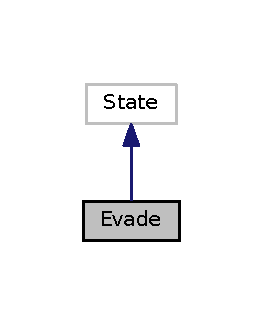
\includegraphics[width=126pt]{classEvade__inherit__graph}
\end{center}
\end{figure}


Collaboration diagram for Evade\+:
\nopagebreak
\begin{figure}[H]
\begin{center}
\leavevmode
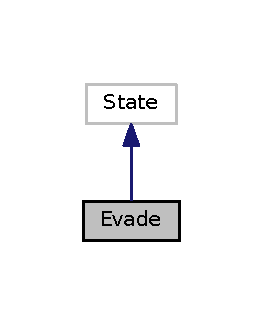
\includegraphics[width=126pt]{classEvade__coll__graph}
\end{center}
\end{figure}
\subsection*{Public Member Functions}
\begin{DoxyCompactItemize}
\item 
\hypertarget{classEvade_ad9069e4cb8ff9a674c6f782e3a993479}{void {\bfseries entry} (const Event \&e)}\label{classEvade_ad9069e4cb8ff9a674c6f782e3a993479}

\item 
\hypertarget{classEvade_ae158ab71688498147b7656fd5f48475d}{void {\bfseries during} ()}\label{classEvade_ae158ab71688498147b7656fd5f48475d}

\item 
\hypertarget{classEvade_aca8e9343f66389858fae7ca9b70d3296}{void {\bfseries exit} (const Event \&e)}\label{classEvade_aca8e9343f66389858fae7ca9b70d3296}

\end{DoxyCompactItemize}


The documentation for this class was generated from the following file\+:\begin{DoxyCompactItemize}
\item 
robot.\+h\end{DoxyCompactItemize}

\hypertarget{classFindRechSta}{\section{Find\+Rech\+Sta Class Reference}
\label{classFindRechSta}\index{Find\+Rech\+Sta@{Find\+Rech\+Sta}}
}


Inheritance diagram for Find\+Rech\+Sta\+:
\nopagebreak
\begin{figure}[H]
\begin{center}
\leavevmode
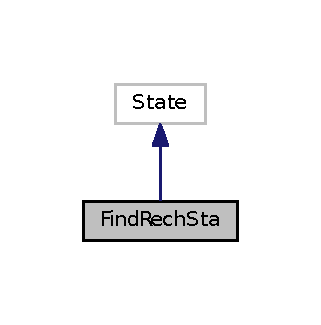
\includegraphics[width=154pt]{classFindRechSta__inherit__graph}
\end{center}
\end{figure}


Collaboration diagram for Find\+Rech\+Sta\+:
\nopagebreak
\begin{figure}[H]
\begin{center}
\leavevmode
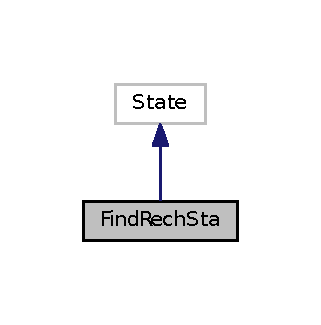
\includegraphics[width=154pt]{classFindRechSta__coll__graph}
\end{center}
\end{figure}
\subsection*{Public Member Functions}
\begin{DoxyCompactItemize}
\item 
\hypertarget{classFindRechSta_a0cf1b5250e971482f267063bc83128c8}{void {\bfseries entry} (const Event \&e)}\label{classFindRechSta_a0cf1b5250e971482f267063bc83128c8}

\item 
\hypertarget{classFindRechSta_a72325611ca2d1c8a4b5d5ffefe6ff058}{void {\bfseries during} ()}\label{classFindRechSta_a72325611ca2d1c8a4b5d5ffefe6ff058}

\item 
\hypertarget{classFindRechSta_add1af0576c619b20c596741aec4b4367}{void {\bfseries exit} (const Event \&e)}\label{classFindRechSta_add1af0576c619b20c596741aec4b4367}

\end{DoxyCompactItemize}


The documentation for this class was generated from the following file\+:\begin{DoxyCompactItemize}
\item 
robot.\+h\end{DoxyCompactItemize}

\hypertarget{classIdle}{\section{Idle Class Reference}
\label{classIdle}\index{Idle@{Idle}}
}


Inheritance diagram for Idle\+:
\nopagebreak
\begin{figure}[H]
\begin{center}
\leavevmode
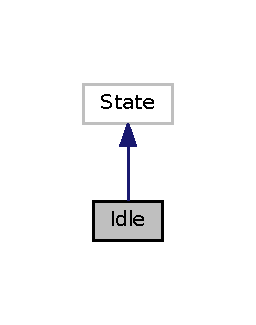
\includegraphics[width=123pt]{classIdle__inherit__graph}
\end{center}
\end{figure}


Collaboration diagram for Idle\+:
\nopagebreak
\begin{figure}[H]
\begin{center}
\leavevmode
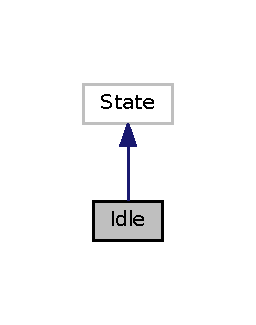
\includegraphics[width=123pt]{classIdle__coll__graph}
\end{center}
\end{figure}
\subsection*{Public Member Functions}
\begin{DoxyCompactItemize}
\item 
\hypertarget{classIdle_abe8c7b8e0551be3c8f055330d256e365}{void {\bfseries entry} (const Event \&e)}\label{classIdle_abe8c7b8e0551be3c8f055330d256e365}

\item 
\hypertarget{classIdle_a68789ed7b16a10ac60a7e1bc44745476}{void {\bfseries during} ()}\label{classIdle_a68789ed7b16a10ac60a7e1bc44745476}

\item 
\hypertarget{classIdle_aaecc780082c26be016105ec98c44a3c6}{void {\bfseries exit} (const Event \&e)}\label{classIdle_aaecc780082c26be016105ec98c44a3c6}

\end{DoxyCompactItemize}


The documentation for this class was generated from the following file\+:\begin{DoxyCompactItemize}
\item 
robot.\+h\end{DoxyCompactItemize}

\hypertarget{classIntruder}{\section{Intruder Class Reference}
\label{classIntruder}\index{Intruder@{Intruder}}
}


Inheritance diagram for Intruder\+:
\nopagebreak
\begin{figure}[H]
\begin{center}
\leavevmode
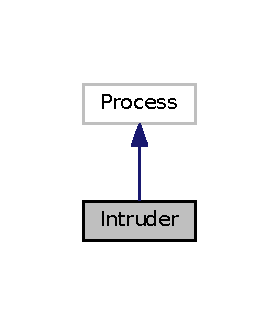
\includegraphics[width=134pt]{classIntruder__inherit__graph}
\end{center}
\end{figure}


Collaboration diagram for Intruder\+:
\nopagebreak
\begin{figure}[H]
\begin{center}
\leavevmode
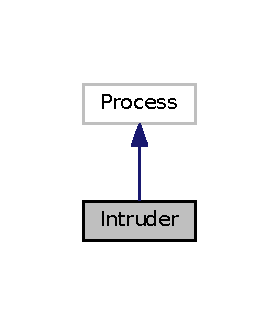
\includegraphics[width=134pt]{classIntruder__coll__graph}
\end{center}
\end{figure}
\subsection*{Public Member Functions}
\begin{DoxyCompactItemize}
\item 
\hypertarget{classIntruder_a38e5fdfbecaa4a3b7f9e927631422ffc}{void {\bfseries init} ()}\label{classIntruder_a38e5fdfbecaa4a3b7f9e927631422ffc}

\item 
\hypertarget{classIntruder_affa4e38dfc67f72e4f551351698be7b6}{void {\bfseries start} ()}\label{classIntruder_affa4e38dfc67f72e4f551351698be7b6}

\item 
\hypertarget{classIntruder_a286f987e30fecdb59a7eb12776891f7d}{void {\bfseries update} ()}\label{classIntruder_a286f987e30fecdb59a7eb12776891f7d}

\item 
\hypertarget{classIntruder_a4bd6180c90d70ec2d6d3067bdf65bf2e}{void {\bfseries stop} ()}\label{classIntruder_a4bd6180c90d70ec2d6d3067bdf65bf2e}

\end{DoxyCompactItemize}


The documentation for this class was generated from the following file\+:\begin{DoxyCompactItemize}
\item 
robot.\+h\end{DoxyCompactItemize}

\hypertarget{classKill}{\section{Kill Class Reference}
\label{classKill}\index{Kill@{Kill}}
}


Inheritance diagram for Kill\+:
\nopagebreak
\begin{figure}[H]
\begin{center}
\leavevmode
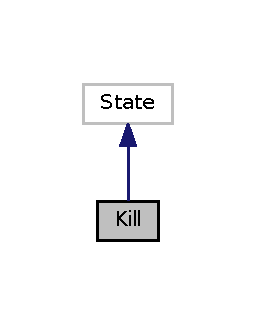
\includegraphics[width=123pt]{classKill__inherit__graph}
\end{center}
\end{figure}


Collaboration diagram for Kill\+:
\nopagebreak
\begin{figure}[H]
\begin{center}
\leavevmode
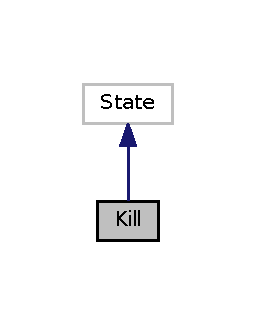
\includegraphics[width=123pt]{classKill__coll__graph}
\end{center}
\end{figure}
\subsection*{Public Member Functions}
\begin{DoxyCompactItemize}
\item 
\hypertarget{classKill_a6f43009a892f30e16cb252c4ddf9d09f}{void {\bfseries entry} (const Event \&e)}\label{classKill_a6f43009a892f30e16cb252c4ddf9d09f}

\item 
\hypertarget{classKill_ac810d887bcc6fe8ef7f1b7ad5cfafffe}{void {\bfseries during} ()}\label{classKill_ac810d887bcc6fe8ef7f1b7ad5cfafffe}

\item 
\hypertarget{classKill_af198d4b7cf0554046d7f5f4687603c72}{void {\bfseries exit} (const Event \&e)}\label{classKill_af198d4b7cf0554046d7f5f4687603c72}

\end{DoxyCompactItemize}


The documentation for this class was generated from the following file\+:\begin{DoxyCompactItemize}
\item 
robot.\+h\end{DoxyCompactItemize}

\hypertarget{classMakeNoise}{\section{Make\+Noise Class Reference}
\label{classMakeNoise}\index{Make\+Noise@{Make\+Noise}}
}


Inheritance diagram for Make\+Noise\+:
\nopagebreak
\begin{figure}[H]
\begin{center}
\leavevmode
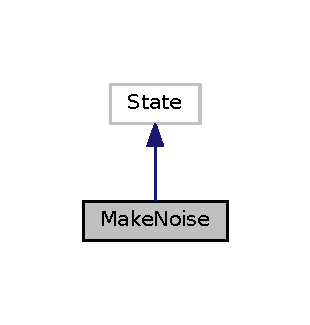
\includegraphics[width=149pt]{classMakeNoise__inherit__graph}
\end{center}
\end{figure}


Collaboration diagram for Make\+Noise\+:
\nopagebreak
\begin{figure}[H]
\begin{center}
\leavevmode
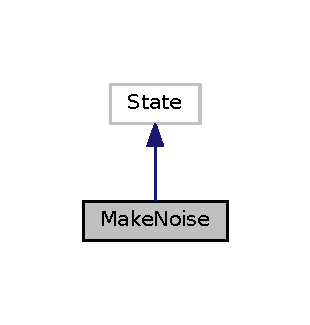
\includegraphics[width=149pt]{classMakeNoise__coll__graph}
\end{center}
\end{figure}
\subsection*{Public Member Functions}
\begin{DoxyCompactItemize}
\item 
\hypertarget{classMakeNoise_a30f1a1e0d701b910521e0d348332d277}{void {\bfseries entry} (const Event \&e)}\label{classMakeNoise_a30f1a1e0d701b910521e0d348332d277}

\item 
\hypertarget{classMakeNoise_a9631c7b76aab917d348a381ac70c9e09}{void {\bfseries during} ()}\label{classMakeNoise_a9631c7b76aab917d348a381ac70c9e09}

\item 
\hypertarget{classMakeNoise_a3857af8ef3595b9cdafcbb790a842a21}{void {\bfseries exit} (const Event \&e)}\label{classMakeNoise_a3857af8ef3595b9cdafcbb790a842a21}

\end{DoxyCompactItemize}


The documentation for this class was generated from the following file\+:\begin{DoxyCompactItemize}
\item 
robot.\+h\end{DoxyCompactItemize}

\hypertarget{classMap}{\section{Map Class Reference}
\label{classMap}\index{Map@{Map}}
}


Inheritance diagram for Map\+:
\nopagebreak
\begin{figure}[H]
\begin{center}
\leavevmode
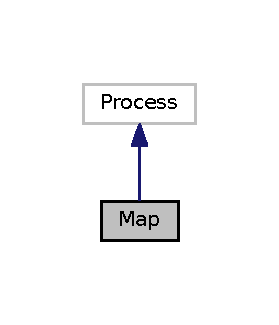
\includegraphics[width=134pt]{classMap__inherit__graph}
\end{center}
\end{figure}


Collaboration diagram for Map\+:
\nopagebreak
\begin{figure}[H]
\begin{center}
\leavevmode
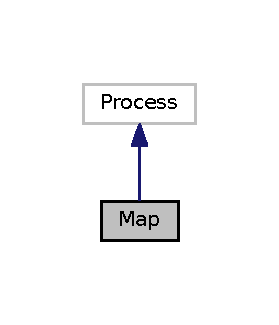
\includegraphics[width=134pt]{classMap__coll__graph}
\end{center}
\end{figure}
\subsection*{Public Member Functions}
\begin{DoxyCompactItemize}
\item 
\hypertarget{classMap_a546e80c365e0ceda9c4ac3777d9648a5}{void {\bfseries Up} (int \&row)}\label{classMap_a546e80c365e0ceda9c4ac3777d9648a5}

\item 
\hypertarget{classMap_a767871d244385ace101d441d3e861be0}{void {\bfseries Down} (int \&row)}\label{classMap_a767871d244385ace101d441d3e861be0}

\item 
\hypertarget{classMap_a07d6a92d5e28921bc4cb85fab86e38d5}{void {\bfseries Left} (int \&col)}\label{classMap_a07d6a92d5e28921bc4cb85fab86e38d5}

\item 
\hypertarget{classMap_a27df7df3064192b2d88d6de45a1d3a4b}{void {\bfseries Right} (int \&col)}\label{classMap_a27df7df3064192b2d88d6de45a1d3a4b}

\item 
\hypertarget{classMap_aa804b353e131db3353887e4403bb7198}{vector$<$ vector$<$ char $>$ $>$ {\bfseries initial\+Map} (int row, int col)}\label{classMap_aa804b353e131db3353887e4403bb7198}

\item 
\hypertarget{classMap_a485f842fd1ccbedcee05eb0c16c10145}{void {\bfseries post\+Map} (vector$<$ vector$<$ char $>$$>$ map)}\label{classMap_a485f842fd1ccbedcee05eb0c16c10145}

\item 
\hypertarget{classMap_a78d03e2c885923d5694ac0ce45e39fe4}{void {\bfseries update\+Map} (vector$<$ vector$<$ char $>$$>$ \&map, \hyperlink{classObj}{Obj} \&r, \hyperlink{classObj}{Obj} \&c)}\label{classMap_a78d03e2c885923d5694ac0ce45e39fe4}

\item 
\hypertarget{classMap_a4fade8eb8d572b68d6f8085983a72f91}{void {\bfseries wander} (vector$<$ vector$<$ char $>$$>$ \&map, \hyperlink{classObj}{Obj} \&r)}\label{classMap_a4fade8eb8d572b68d6f8085983a72f91}

\item 
\hypertarget{classMap_ae3a387c6842c05596b004e2735b8cbf5}{void {\bfseries init} ()}\label{classMap_ae3a387c6842c05596b004e2735b8cbf5}

\item 
\hypertarget{classMap_acb55c5346f6e0948635a72d7071004ef}{void {\bfseries start} ()}\label{classMap_acb55c5346f6e0948635a72d7071004ef}

\item 
\hypertarget{classMap_ab12643cc3a8d5e48f566c1abb571e9bf}{void {\bfseries update} ()}\label{classMap_ab12643cc3a8d5e48f566c1abb571e9bf}

\item 
\hypertarget{classMap_ab8412a04e493f4efef5327ed86209317}{void {\bfseries stop} ()}\label{classMap_ab8412a04e493f4efef5327ed86209317}

\end{DoxyCompactItemize}


The documentation for this class was generated from the following file\+:\begin{DoxyCompactItemize}
\item 
robot.\+h\end{DoxyCompactItemize}

\hypertarget{classObj}{\section{Obj Class Reference}
\label{classObj}\index{Obj@{Obj}}
}
\subsection*{Public Member Functions}
\begin{DoxyCompactItemize}
\item 
\hypertarget{classObj_a6bd434ff444808f507e73868e1a3811e}{void {\bfseries random} ()}\label{classObj_a6bd434ff444808f507e73868e1a3811e}

\item 
\hypertarget{classObj_ab626ae12167372b1432c871842279e78}{void {\bfseries set} (int ir, int ic)}\label{classObj_ab626ae12167372b1432c871842279e78}

\end{DoxyCompactItemize}
\subsection*{Public Attributes}
\begin{DoxyCompactItemize}
\item 
\hypertarget{classObj_a8371ea5021c815b409eabcbafc1cc674}{int {\bfseries row}}\label{classObj_a8371ea5021c815b409eabcbafc1cc674}

\item 
\hypertarget{classObj_ad6fe3e1c1129967f4ad9e225d5ac2e79}{int {\bfseries col}}\label{classObj_ad6fe3e1c1129967f4ad9e225d5ac2e79}

\end{DoxyCompactItemize}


The documentation for this class was generated from the following file\+:\begin{DoxyCompactItemize}
\item 
robot.\+h\end{DoxyCompactItemize}

\hypertarget{classReChar}{\section{Re\+Char Class Reference}
\label{classReChar}\index{Re\+Char@{Re\+Char}}
}


Inheritance diagram for Re\+Char\+:
\nopagebreak
\begin{figure}[H]
\begin{center}
\leavevmode
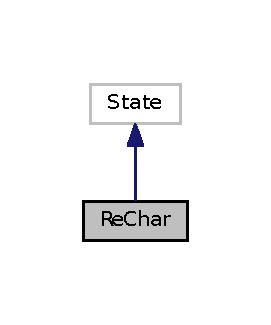
\includegraphics[width=130pt]{classReChar__inherit__graph}
\end{center}
\end{figure}


Collaboration diagram for Re\+Char\+:
\nopagebreak
\begin{figure}[H]
\begin{center}
\leavevmode
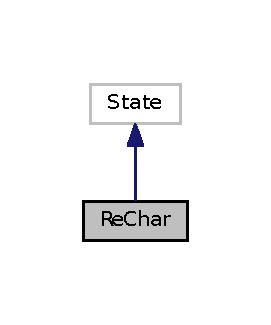
\includegraphics[width=130pt]{classReChar__coll__graph}
\end{center}
\end{figure}
\subsection*{Public Member Functions}
\begin{DoxyCompactItemize}
\item 
\hypertarget{classReChar_a0f36c7acbe46cc2a9e7907d1555e255c}{void {\bfseries entry} (const Event \&e)}\label{classReChar_a0f36c7acbe46cc2a9e7907d1555e255c}

\item 
\hypertarget{classReChar_a7d1f1896d9b2dcf3c74ec244f404be02}{void {\bfseries during} ()}\label{classReChar_a7d1f1896d9b2dcf3c74ec244f404be02}

\item 
\hypertarget{classReChar_afdee4daa56738277b0e29ef220cbb870}{void {\bfseries exit} (const Event \&e)}\label{classReChar_afdee4daa56738277b0e29ef220cbb870}

\end{DoxyCompactItemize}


The documentation for this class was generated from the following file\+:\begin{DoxyCompactItemize}
\item 
robot.\+h\end{DoxyCompactItemize}

\hypertarget{classRobot}{\section{Robot Class Reference}
\label{classRobot}\index{Robot@{Robot}}
}


Inheritance diagram for Robot\+:
\nopagebreak
\begin{figure}[H]
\begin{center}
\leavevmode
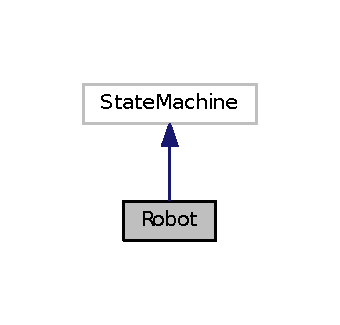
\includegraphics[width=163pt]{classRobot__inherit__graph}
\end{center}
\end{figure}


Collaboration diagram for Robot\+:
\nopagebreak
\begin{figure}[H]
\begin{center}
\leavevmode
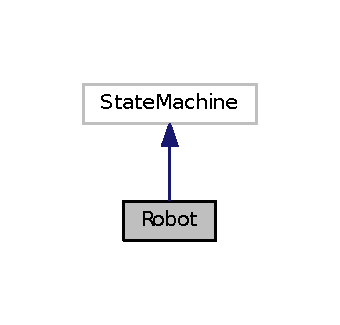
\includegraphics[width=163pt]{classRobot__coll__graph}
\end{center}
\end{figure}
\subsection*{Public Member Functions}
\begin{DoxyCompactItemize}
\item 
\hypertarget{classRobot_a76bf162c87054d8f1b3c6e1656caf46b}{{\bfseries Robot} (std\+::string name)}\label{classRobot_a76bf162c87054d8f1b3c6e1656caf46b}

\end{DoxyCompactItemize}
\subsection*{Public Attributes}
\begin{DoxyCompactItemize}
\item 
\hypertarget{classRobot_a932d0cd136fe1c245452740141526825}{friend {\bfseries Map}}\label{classRobot_a932d0cd136fe1c245452740141526825}

\end{DoxyCompactItemize}


The documentation for this class was generated from the following file\+:\begin{DoxyCompactItemize}
\item 
robot.\+h\end{DoxyCompactItemize}

\hypertarget{classWander}{\section{Wander Class Reference}
\label{classWander}\index{Wander@{Wander}}
}


Inheritance diagram for Wander\+:
\nopagebreak
\begin{figure}[H]
\begin{center}
\leavevmode
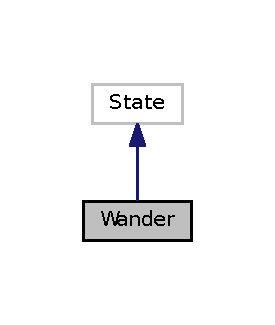
\includegraphics[width=132pt]{classWander__inherit__graph}
\end{center}
\end{figure}


Collaboration diagram for Wander\+:
\nopagebreak
\begin{figure}[H]
\begin{center}
\leavevmode
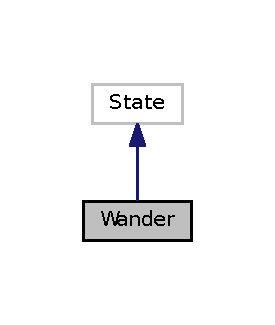
\includegraphics[width=132pt]{classWander__coll__graph}
\end{center}
\end{figure}
\subsection*{Public Member Functions}
\begin{DoxyCompactItemize}
\item 
\hypertarget{classWander_a977a4089a2767ad5b6674f18b3a28838}{void {\bfseries entry} (const Event \&e)}\label{classWander_a977a4089a2767ad5b6674f18b3a28838}

\item 
\hypertarget{classWander_ae2cd859893ca9b40313e25440c83787a}{void {\bfseries during} ()}\label{classWander_ae2cd859893ca9b40313e25440c83787a}

\item 
\hypertarget{classWander_a7b8cbd71ac448d7228d6bd4716fca720}{void {\bfseries exit} (const Event \&e)}\label{classWander_a7b8cbd71ac448d7228d6bd4716fca720}

\end{DoxyCompactItemize}


The documentation for this class was generated from the following file\+:\begin{DoxyCompactItemize}
\item 
robot.\+h\end{DoxyCompactItemize}

%--- End generated contents ---

% Index
\newpage
\phantomsection
\addcontentsline{toc}{chapter}{Index}
\printindex

\end{document}
